\section{Introduction}

\subsection{Motivation}
Visualizations on paper vs on PowerPoint, new media purposefully used. This thesis draws inspiration, but no theory or code from Khan Academy and the Python-based mathematics visualization library \texttt{manim}\footnote{https://github.com/3b1b/manim}.

\subsection{Goal of this Thesis}
to visualize algorithms from in specific instances.

The domain of query optimization poses many algorithms that can be visualized well.

However, visualizing algorithms can provide far more than just merely helping students understand the intricate concepts better.
Among professional computer scientists and software engineers the visualization of algorithms has proven a useful debugging and exploration technique.

In this Master thesis, I want to provide a generic toolset for algorithms. I aim for a framework that lets you generate the visualizations in a generic way—no explicit drawing is needed.

Instead of investigating what the constitutents of an algorithm \textit{could} be and
implementing them accordingly, we use a top-down approach and implement the steps of
two pre-chosen algorithms, namely \texttt{DPccp} \cite{moerkotte2006analysis} and Adaptive Radix Trees \cite{leis2013adaptive}.

Lack of good tooling in database algorithm development.
Visual debugging and aids more commonplace.
\begin{figure}
    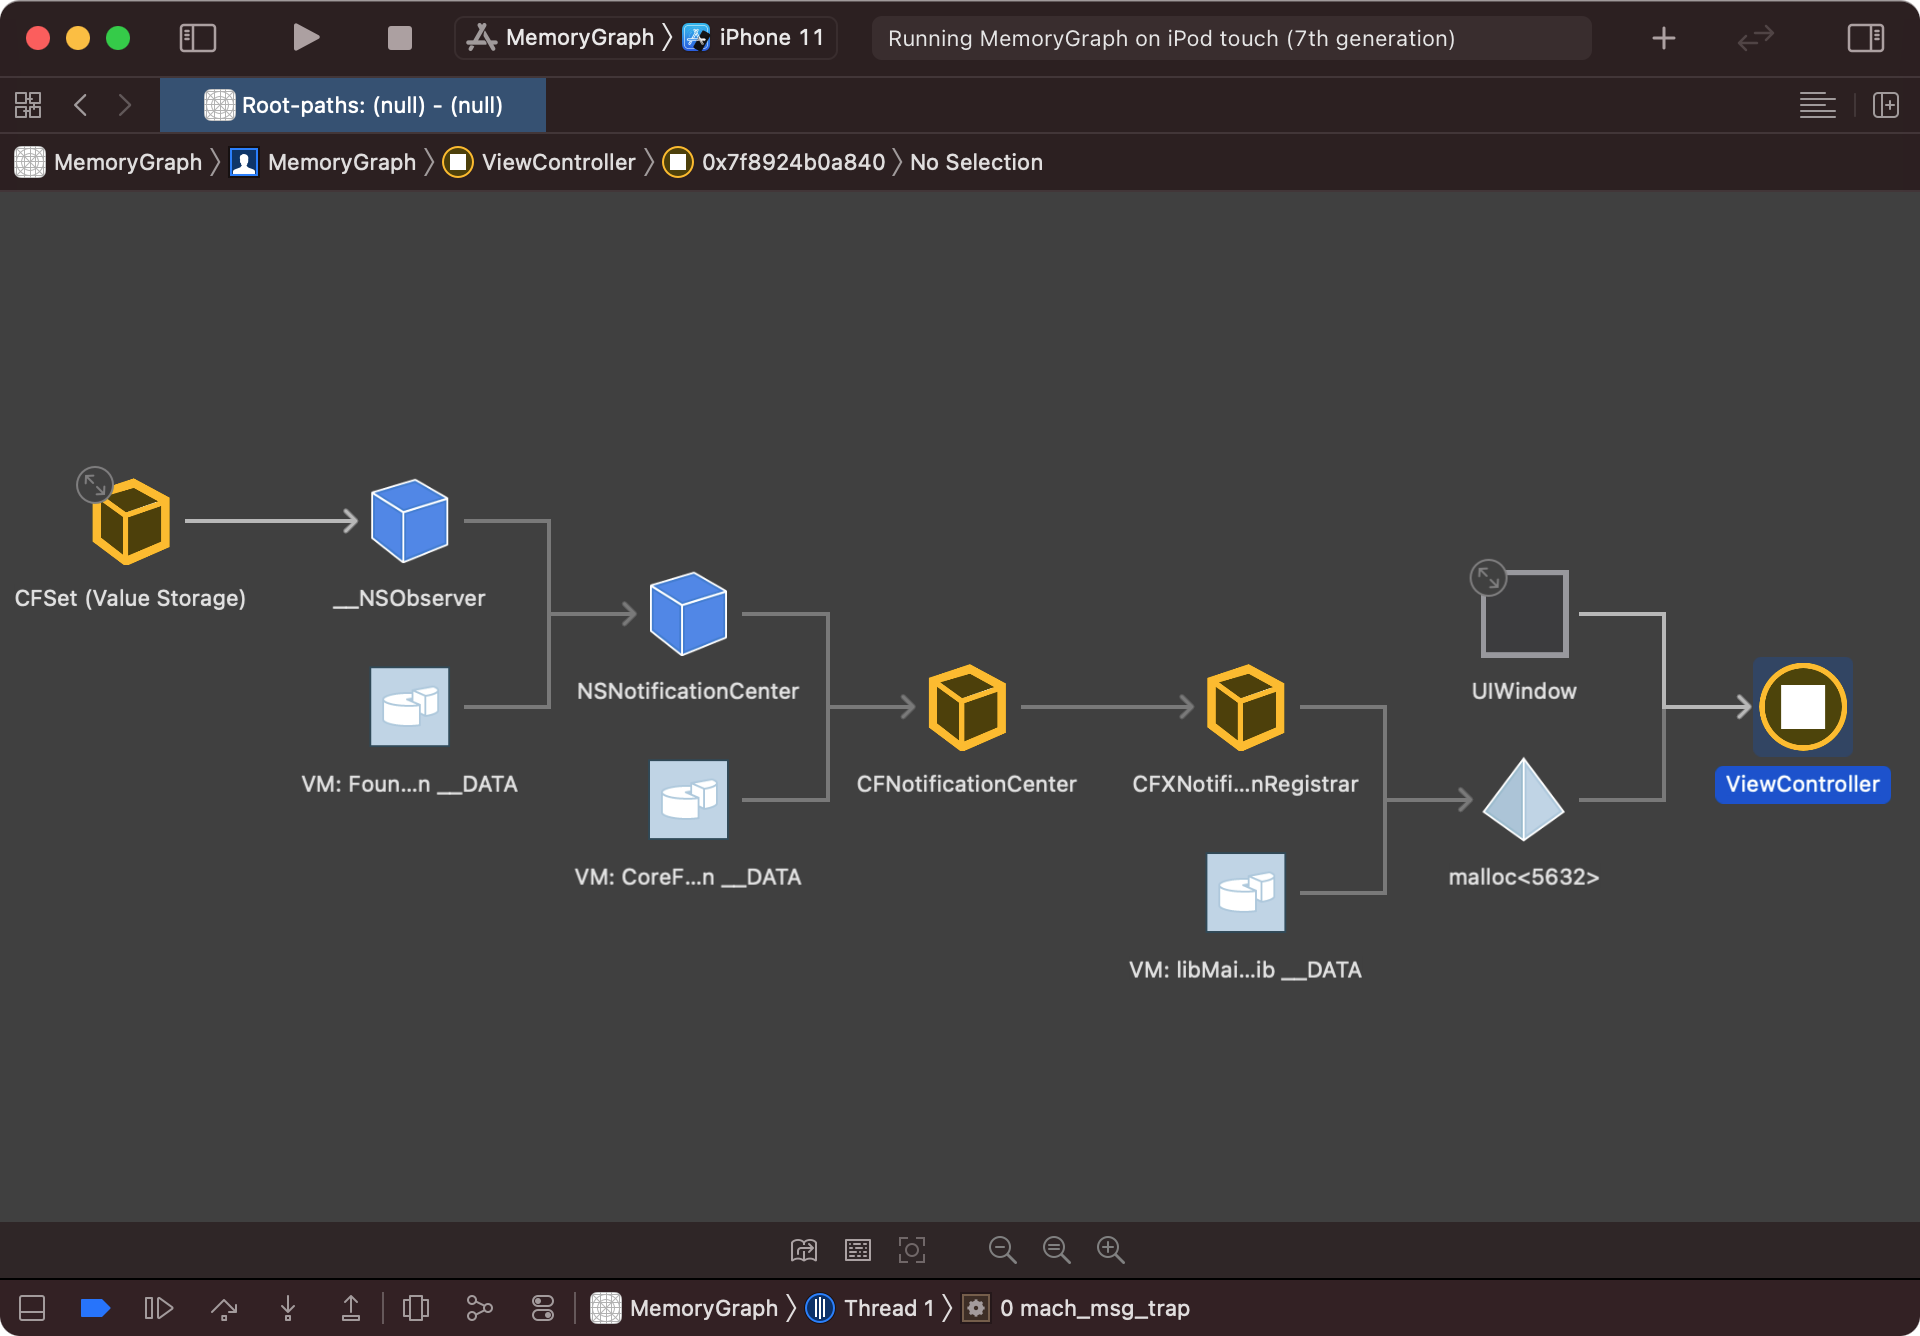
\includegraphics[width=\textwidth]{img/memoryGraph.png}
    \caption{Memory graph in Xcode 12}
\end{figure}


\subsection{Prior Art}
